\documentclass[aspectratio=1610]{beamer}
\usetheme{bjeldbak}
\usepackage{xspace}
\usepackage{graphicx}
\usepackage{textpos}
\usepackage{subfigure}
\usepackage{pifont}
\usepackage[super]{nth}
\usepackage{relsize}
\usepackage{amsmath}
\usepackage{bm}

\setbeamertemplate{section page}{
  \begin{centering}
    \begin{beamercolorbox}[sep=12pt,center]{part title}
      \huge
      \insertsection
    \end{beamercolorbox}
  \end{centering}
}

\definecolor{anti-flashwhite}{rgb}{0.95, 0.95, 0.96}

\setbeamercolor{section in toc}{fg=anti-flashwhite}

\setbeamertemplate{section page}{
  \begin{centering}
    \begin{beamercolorbox}[sep=12pt,center]{part title}
      \huge
      \insertsection
    \end{beamercolorbox}
  \end{centering}
}

\usepackage{ifthen}
\usepackage{mciteplus} 
\newboolean{uprightparticles}
\setboolean{uprightparticles}{false} %Set true for upright particle symbols
\usepackage{xspace} 
\usepackage{upgreek}

\input{lhcb-symbols-def}
\input{spd-symbols-def}
\input{tracking-symbols-def}

\def \Cseven {\ensuremath{\mathcal{C}_{7}^{(\ensuremath{\prime})}}\xspace}
\def \Cnine {\ensuremath{\mathcal{C}_{9}^{(\ensuremath{\prime})}}\xspace}
\def \Cten {\ensuremath{\mathcal{C}_{10}^{(\ensuremath{\prime})}}\xspace}
\def \Cnineten {\ensuremath{\mathcal{C}_{9,10}^{(\ensuremath{\prime})}}\xspace}

\usepackage{appendixnumberbeamer}
\expandafter\def\expandafter\insertshorttitle\expandafter{%
  \insertshorttitle\hfill\insertframenumber\,/\,\inserttotalframenumber}

\usepackage[linewidth=1pt]{mdframed}
\newenvironment{myenv}[1]
{\mdfsetup{
  frametitle={\colorbox{white}{\space#1\space}},
  innertopmargin=3pt,
  frametitleaboveskip=-\ht\strutbox,
  frametitlealignment=\center
}
\begin{mdframed}%
}
{\end{mdframed}}

\setbeamertemplate{blocks}[rounded][shadow=false]
\setbeamercolor{block body}{bg=barcolor!40,fg=black}
\setbeamercolor{block title}{bg=barcolor!20,fg=black}

\usepackage{tikz}
\usetikzlibrary{shapes,arrows}

\definecolor{babyblue}{rgb}{0.54, 0.81, 0.94}
\definecolor{byzantine}{rgb}{0.74, 0.2, 0.64}
\definecolor{anti-flashwhite}{rgb}{0.95, 0.95, 0.96}
\definecolor{burgundy}{rgb}{0.5, 0.0, 0.13}
\definecolor{burntorange}{rgb}{0.8, 0.33, 0.0}
\definecolor{cadmiumorange}{rgb}{0.93, 0.53, 0.18}
\definecolor{bleudefrance}{rgb}{0.19, 0.55, 0.91}
\definecolor{bostonuniversityred}{rgb}{0.8, 0.0, 0.0}
\definecolor{darkred}{rgb}{0.55, 0.0, 0.0}
\definecolor{blue(ryb)}{rgb}{0.01, 0.28, 1.0}
\definecolor{darkgreen}{rgb}{0.0, 0.5, 0.0}
\definecolor{palatinatepurple}{rgb}{0.41, 0.16, 0.38}
\definecolor{cadmiumorange}{rgb}{0.93, 0.53, 0.18}
\definecolor{airforceblue}{rgb}{0.36, 0.54, 0.66}
\definecolor{ceruleanblue}{rgb}{0.16, 0.32, 0.75}
\definecolor{applegreen}{rgb}{0.55, 0.71, 0.0}
\definecolor{antiquebrass}{rgb}{0.8, 0.58, 0.46}
\definecolor{cobalt}{rgb}{0.0, 0.28, 0.67}
\definecolor{darkorchid}{rgb}{0.6, 0.2, 0.8}
\definecolor{darkpastelgreen}{rgb}{0.01, 0.75, 0.24}
\definecolor{darkpastelred}{rgb}{0.76, 0.23, 0.13}
\definecolor{darkspringgreen}{rgb}{0.09, 0.45, 0.27}

\def\KstarP  {\ensuremath{\kaon^{*}(892)^{0}}\xspace}
\def\Kstarfourteenthirty  {{\ensuremath{\kaon^{*}_{0,2}(1430)^{0}}}\xspace}
\DeclareRobustCommand{\orderof}{\ensuremath{\mathcal{O}}}
\usepackage[export]{adjustbox}

\tikzset{
  every overlay node/.style={
    draw=white,anchor=north west,
  },
}
\def\tikzoverlay{%
   \tikz[baseline,overlay]\node[every overlay node]
}%

%%%%%%%%%%%%%%%%%%%%%%%%%%%%%%%%%%%%%%%%%%%%%%%%%%%%%%%%%%%%%%%%%
%Begin document
%%%%%%%%%%%%%%%%%%%%%%%%%%%%%%%%%%%%%%%%%%%%%%%%%%%%%%%%%%%%%%%%%
\begin{document}
\title[]{Upstream Tracking and the Decay $\B^{0} \to K^{+}\pi^{-}\mu^{+}\mu^{-}$\\ at the LHCb Experiment}
\author[Espen Eie Bowen]{{\bf Espen Eie Bowen} \\ {\small PhD defense}} 
\institute[]{}
\date{\nth{19} January 2017}
%%%%%%%%%%%%%%%%%%%%%%%%%%%%%%%%%%%%%%%%%%%%%%%%%%%%%%%%%%%%%%%%%
%Title
%%%%%%%%%%%%%%%%%%%%%%%%%%%%%%%%%%%%%%%%%%%%%%%%%%%%%%%%%%%%%%%%%
\begin{frame}[plain]
\titlepage
\begin{textblock*}{2cm}(12.5cm,0.0cm)
  \includegraphics[width=2cm]{figs/lhcb-logo.pdf}
\end{textblock*}
\begin{textblock*}{5cm}(0.0cm,0.0cm)
  \includegraphics[width=3.0cm]{figs/uzh.jpg}
\end{textblock*}
\end{frame}

%%%%%%%%%%%%%%%%%%%%%%%%%%%%%%%%%%%%%%%%%%%%%%%%%%%%%%%%%%%%%%%%%
%Slide
%%%%%%%%%%%%%%%%%%%%%%%%%%%%%%%%%%%%%%%%%%%%%%%%%%%%%%%%%%%%%%%%%
\begin{frame}{The \lhcb experiment}
  \begin{itemize}
  \item LHCb is the dedicated heavy flavour physics experiment at the LHC
  \item Its primary goal is to look for indirect evidence of new physics in $CP$ violation and rare decays of beauty and charm hadrons
  \item This requires:
    \begin{enumerate}
    \item Excellent tracking 
      \begin{itemize}
      \item momentum resolution ($\delta p/p \sim 0.4\% - 0.6\%$)
      \item impact parameter resolution ($\sigma_{\rm IP} \sim 20\mum$)
      \item primary vertex resolution (13 \mum in $x$ and $y$ and 71\mum in $z$)
      \end{itemize}
    \item Excellent decay time resolution ($\sigma_{\tau}$ $\sim$ 45\fs)
    \item Excellent particle identification
    \end{enumerate}
  \end{itemize}

  \bigskip
    
  \begin{columns}
    \begin{column}{0.29\textwidth}
      \centering
      \begin{tikzpicture}
        \node[anchor=south west,inner sep=0] at (0,0) {\includegraphics[height=3.5cm]{figs/lhcb/massres.pdf}};
        \node[draw=none,barcolor!80!black] at (1.4,0.15) {\tiny \href{http://link.springer.com/article/10.1007\%2FJHEP06(2013)064}{JHEP 06 (2013) 064}};
      \end{tikzpicture}
    \end{column}
    \begin{column}{0.36\textwidth}
      \centering
      \begin{tikzpicture}
        \node[anchor=south west,inner sep=0] at (0,0) {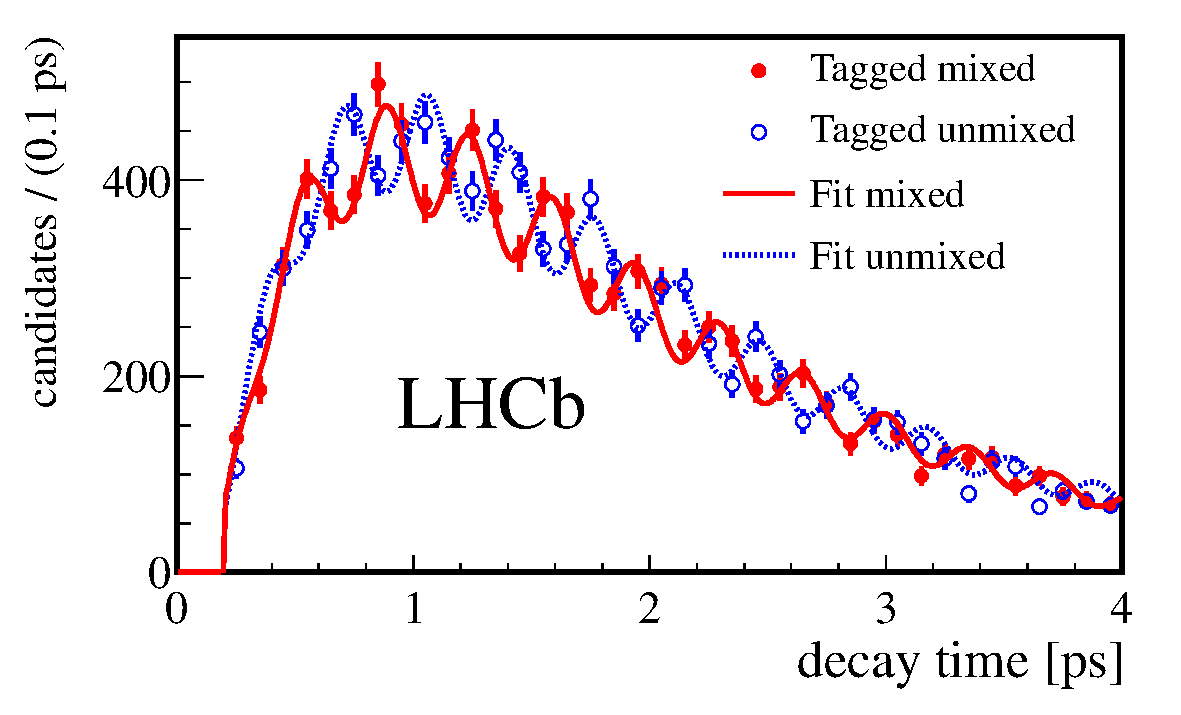
\includegraphics[height=3.5cm]{figs/lhcb/bsmix.pdf}};
        \node[draw=none,barcolor!80!black] at (2.2,0.15) {\tiny \href{http://iopscience.iop.org/1367-2630/15/5/053021/}{New~J.~Phys. 15 (2013) 053021}};
      \end{tikzpicture}
    \end{column}
    \begin{column}{0.36\textwidth}
      \begin{tikzpicture}
        \node[anchor=south west,inner sep=0] at (0,0) {\includegraphics[height=3.5cm]{figs/lhcb/RICH.png}};
        \node[draw=none,barcolor!80!black] at (1.4,0.15) {\tiny \href{http://epjc.epj.org/articles/epjc/abs/2013/05/10052_2013_Article_2431/10052_2013_Article_2431.html}{Eur. Phys. J. C (2013) 73}};
        \end{tikzpicture}
    \end{column}
  \end{columns}
\end{frame}

%%%%%%%%%%%%%%%%%%%%%%%%%%%%%%%%%%%%%%%%%%%%%%%%%%%%%%%%%%%%%%%%%
%Slide
%%%%%%%%%%%%%%%%%%%%%%%%%%%%%%%%%%%%%%%%%%%%%%%%%%%%%%%%%%%%%%%%%
\begin{frame}\frametitle{}
  \begin{center}
    \begin{tikzpicture}
      \node[anchor=south west,inner sep=0](image) at (0,0) {\includegraphics[width=\textwidth]{figs/lhcb/lhcb2.png}};
      
      \begin{scope}[x={(image.south east)},y={(image.north west)}]
        %\draw[help lines,xstep=.1,ystep=.1] (0,0) grid (1,1);
        
        \node[draw=none,burgundy] at (0.15,0.05) {Vertex Locator};
        \draw[ultra thick,->,burgundy] (0.15,0.1) -- (0.2,0.4);
        
        \node[draw=none,cadmiumorange] at (0.20,0.95) {Tracking system (TT, IT, OT)};
        \draw[ultra thick,->,cadmiumorange] (0.14,0.9) -- (0.3,0.48);
        \draw[ultra thick,->,cadmiumorange] (0.14,0.9) -- (0.58,0.52); 
        
        \node[draw=none,byzantine] at (0.49,0.95) {Rich detectors};
        \draw[ultra thick,->,byzantine] (0.5,0.9) -- (0.23,0.55);
        \draw[ultra thick,->,byzantine] (0.5,0.9) -- (0.65,0.65);
        
        \node[draw=none,gray] at (0.45,0.2) {Magnet};
        
        \node[draw=none,babyblue] at (0.7,0.05) {Calorimeters};
        \draw[ultra thick,->,babyblue] (0.7,0.1) -- (0.75,0.55);
        
        \node[draw=none,green!90!black] at (0.9,0.7) {Muon system};
        
      \end{scope}
    \end{tikzpicture}
    
  \end{center}
\end{frame}

%%%%%%%%%%%%%%%%%%%%%%%%%%%%%%%%%%%%%%%%%%%%%%%%%%%%%%%%%%%%%%%%%
%Slide
%%%%%%%%%%%%%%%%%%%%%%%%%%%%%%%%%%%%%%%%%%%%%%%%%%%%%%%%%%%%%%%%%
\begin{frame}{Track reconstruction at \lhcb}

\begin{columns}
\begin{column}{0.5\textwidth}
\begin{itemize}
\item Track reconstruction at \lhcb is performed by several different algorithms
\item Two standalone algorithms 
  \begin{itemize}
    \item[\ding{70}] \velo tracking and T track seeding
  \end{itemize}
\item Other algorithms use input from these to perform further track reconstruction
\item Long tracks used for majority of \lhcb analyses
  \begin{itemize}
    \item[\ding{70}] Traverse the full tracking system
    \begin{itemize}
    \item[$\blacktriangleright$] Best momentum resolution
    \end{itemize}
  \end{itemize}
\end{itemize}
\end{column}
\begin{column}{0.5\textwidth}
\begin{tikzpicture}
\node[anchor=south west,inner sep=0](image) at (0,0) {\includegraphics[trim={1cm 0 2cm 0},clip,width=\textwidth]{figs/tracking/trackTypes.pdf}};
\begin{scope}[x={(image.south east)},y={(image.north west)}]
%\draw[help lines,xstep=.1,ystep=.1] (0,0) grid (1,1);
\fill[white] (0.22,0.58) rectangle (0.29,0.62);
\node at (0.25,0.6) {\footnotesize {\fontfamily{cmss}\selectfont TT}};
\end{scope}
\end{tikzpicture} 
\end{column}
\end{columns}
\end{frame}

%%%%%%%%%%%%%%%%%%%%%%%%%%%%%%%%%%%%%%%%%%%%%%%%%%%%%%%%%%%%%%%%%
%Slide
%%%%%%%%%%%%%%%%%%%%%%%%%%%%%%%%%%%%%%%%%%%%%%%%%%%%%%%%%%%%%%%%%
\begin{frame}{The \lhcb trigger in Run 1}

\begin{columns}
\begin{column}{0.7\textwidth}
   \begin{itemize}
     \item Plays important role in selecting interesting events and rejecting background
   \end{itemize}
\vspace{-0.3cm}
\begin{myenv}{Level 0 Trigger}[linecolor=barcolor]
  \begin{itemize}
    \setlength{\itemindent}{0.5em}
    \item Implemented in hardware
    \item High $p_{T}$ and $E_{T}$ signatures in muon and calorimeter systems
    \item 1 MHz detector readout
  \end{itemize}
\end{myenv}
\vspace{-0.2cm}
\begin{myenv}{Higher Level Trigger}[linecolor=barcolor]
  \begin{itemize}
    \setlength{\itemindent}{0.5em}
      \item Flexible software triggers
%      \item Two stages (HLT1 and HLT2)
      \item Track reconstruction and PV finding performed
        \begin{itemize}
        \item[\ding{70}] Simplified reconstruction w.r.t offline 
        \item[\ding{70}] Preliminary alignment and calibration
        \item[\ding{70}] No RICH PID used
        \end{itemize}
      \item Combination of inclusive and exclusive selections
      \end{itemize}
\end{myenv}
\end{column}
\begin{column}{0.3\textwidth}
\includegraphics[width=\textwidth]{figs/detector/trigger-run1.pdf}
\end{column}
\end{columns}

\end{frame}

%%%%%%%%%%%%%%%%%%%%%%%%%%%%%%%%%%%%%%%%%%%%%%%%%%%%%%%%%%%%%%%%%
%Slide
%%%%%%%%%%%%%%%%%%%%%%%%%%%%%%%%%%%%%%%%%%%%%%%%%%%%%%%%%%%%%%%%%
\begin{frame}{\lhcb Run 2 (2015-2018)}

\begin{columns}
\begin{column}{0.7\textwidth}
\begin{itemize}
  \item \lhcb taking data at $\sqs=13\tev$ and $\lum=4\times10^{32}\cm^{-2}\sec^{-1}$
\end{itemize}

\begin{itemize}
  \item Trigger redesigned with two key objectives
  \begin{enumerate}
      \item Perform full event reconstruction within the trigger
      \item Achieve offline-quality alignment and calibration online
    \end{enumerate}
\end{itemize}

\begin{itemize}
  \item Can perform physics analysis directly on trigger output
  \begin{itemize}
      \item[\ding{70}] Large saving in storage space
      \begin{itemize}
        \item Ideal for analysis of channels with large yield 
      \end{itemize}
      \item[\ding{70}] Allows rapid turn around from data taking to physics analysis
      \begin{itemize}
        \item \orderof(few weeks)
      \end{itemize}
    \end{itemize}
\end{itemize}

\end{column}
\begin{column}{0.3\textwidth}
\includegraphics[width=\textwidth]{figs/detector/trigger-run2.pdf}
\end{column}
\end{columns}

\end{frame}

%%%%%%%%%%%%%%%%%%%%%%%%%%%%%%%%%%%%%%%%%%%%%%%%%%%%%%%%%%%%%%%%%
%Slide
%%%%%%%%%%%%%%%%%%%%%%%%%%%%%%%%%%%%%%%%%%%%%%%%%%%%%%%%%%%%%%%%%
\begin{frame}{The \lhcb Upgrade (2020+)}

\begin{columns}
\begin{column}{0.6\textwidth}
  \begin{itemize}
    \item \lhcb  will undergo upgrade during LS1 (2018-2019) to allow data taking at \mbox{$\sqs=14\tev$ and $\lum=2\times10^{33}\cm^{-2}\sec^{-1}$}
  \end{itemize}

  \begin{itemize}
    \item Two key features
    \begin{enumerate}
      \item Triggerless readout
      \begin{itemize}
        \item[\ding{70}] Remove L0 trigger bottleneck
        \item[\ding{70}] Read out detector at 40\mhz
      \end{itemize}
      \item Full software trigger
      \begin{itemize}
        \item[\ding{70}] Full event reconstruction
        \item[\ding{70}] Offers great flexibility for designing selections
        \item[\ding{70}] Increases trigger efficiency for many physics channels
        \item[\ding{80}] Strict requirements on execution time of tracking algorithms
      \end{itemize}
    \end{enumerate}
  \end{itemize}

  \begin{itemize}
    \item Front end electronics need to be replaced
    \item Many existing sub-detectors will be upgraded
    \begin{itemize}
        \item[\ding{70}] e.g. TT replaced by UT
      \end{itemize}
  \end{itemize}

\end{column}
\begin{column}{0.4\textwidth}
\centering
\vspace{-1cm}
\adjincludegraphics[width=\textwidth,trim={{.3\width} {.575\height} {.28\width} {.1\height}},clip]{figs/detector/upgrade-motivation.pdf}
\includegraphics[width=0.8\textwidth]{figs/detector/UT.pdf}
\end{column}

\end{columns}

\end{frame}

%%%%%%%%%%%%%%%%%%%%%%%%%%%%%%%%%%%%%%%%%%%%%%%%%%%%%%%%%%%%%%%%%
%Slide
%%%%%%%%%%%%%%%%%%%%%%%%%%%%%%%%%%%%%%%%%%%%%%%%%%%%%%%%%%%%%%%%%
\begin{frame}{Novel idea: Upstream tracking for the Upgrade}
\begin{itemize}
  \item Upstream tracks could the speed up the tracking sequence of the Upgrade software trigger
  \item Advantages over using VELO tracks
    \begin{itemize}
      \item Charge and momentum of track segment ($\delta \ptot/\ptot \sim 15 \%$)
      \begin{itemize}
        \item[\ding{212}] Preselect on track \pt
        \item[\ding{212}] Open smaller search windows
        \item[\ding{70}] Greatly reduce execution time and ghost rate!
      \end{itemize}
    \end{itemize}
  \end{itemize}

  \begin{center}
  \input{figs/tikz/upstream-tracking-upgrade-search-window}
  \end{center}

  \begin{itemize}
  \item Upstream tracking algorithm needs to be both fast and efficient
  \end{itemize}
\end{frame}

%%%%%%%%%%%%%%%%%%%%%%%%%%%%%%%%%%%%%%%%%%%%%%%%%%%%%%%%%%%%%%%%%
%Slide
%%%%%%%%%%%%%%%%%%%%%%%%%%%%%%%%%%%%%%%%%%%%%%%%%%%%%%%%%%%%%%%%%
\begin{frame}\frametitle{Upstream tracking (VeloTT) in Run 1}
  \begin{itemize}
  \item[$\blacktriangleright$] Linearly extrapolate VELO track to TT
  \item[$\blacktriangleright$] Open search windows in each layer and find $\Delta x$ between track and hits
  \item[$\blacktriangleright$] Scale $\Delta x$ to reference plane at center of TT
  \item[$\blacktriangleright$] Choose clusters of hits consistent with coming from the same VELO track
  \begin{itemize}
    \item[\ding{80}] Each hit must be on the same side of the linear extrapolation
  \end{itemize}
  \item[$\blacktriangleright$] Fit each track candidate with a simple $\chi^{2}$ fit
  \item[$\blacktriangleright$] Choose best candidate track based on \mbox{\# layers} fired and $\chi^{2}$
  \item[\ding{80}] Fit track with full Kalman filter
  \end{itemize}
  \input{figs/tikz/tracking-velott}
\end{frame}

%%%%%%%%%%%%%%%%%%%%%%%%%%%%%%%%%%%%%%%%%%%%%%%%%%%%%%%%%%%%%%%%%
%Slide
%%%%%%%%%%%%%%%%%%%%%%%%%%%%%%%%%%%%%%%%%%%%%%%%%%%%%%%%%%%%%%%%%
\begin{frame}{VeloUT: Initial peformance}

\begin{columns}
\begin{column}{0.65\textwidth}

\begin{itemize}
  \item Initial version of VeloUT a replication of VeloTT algorithm from Run 1
\end{itemize}

\begin{itemize}
  \item Execution time of 27.20\ms far too slow use in the software trigger
  \begin{itemize}
    \item[\ding{70}] c.f. VELO tracking $\sim1.8\ms$
  \end{itemize}
  \item Reconstruction efficiency too low
  \begin{itemize}
    \item[\ding{70}] Any inefficiency will be propagated to next step
    \item[\ding{70}] Decreases as a function of \ptot
  \end{itemize}
\end{itemize}

\bigskip

\begin{mdframed}[linecolor=barcolor]
\begin{center}
\resizebox{\columnwidth}{!}{
\begin{tabular}{c|c|c|c}
  \velout & Efficiency [\%] & Ghost rate [\%] & Timing [ms] \\ 
  \hline
  v1r2  & 93.94  & 7.21  &  27.20  \\
 \end{tabular}
 }
\end{center}
\end{mdframed}
\end{column}

\begin{column}{0.35\textwidth}
\centering
\begin{figure}
\vspace*{-1cm}
\includegraphics[height=0.475\textheight]{figs/upstream-tracking-upgrade/eff_p_v1r2.pdf}\\
\includegraphics[height=0.475\textheight]{figs/upstream-tracking-upgrade/gr_p_v1r2.pdf}
\end{figure}
\end{column}
\end{columns}

\end{frame}

%%%%%%%%%%%%%%%%%%%%%%%%%%%%%%%%%%%%%%%%%%%%%%%%%%%%%%%%%%%%%%%%%
%Slide
%%%%%%%%%%%%%%%%%%%%%%%%%%%%%%%%%%%%%%%%%%%%%%%%%%%%%%%%%%%%%%%%%
\begin{frame}{VeloUT: Improvements}

\begin{myenv}{Efficiency too low/falls off with increasing \ptot}[linecolor=barcolor]
  \begin{itemize}
    \setlength{\itemindent}{0.5em}
    \item[$\blacktriangleright$] Tracked down to poor assumptions made when associating hits to \velo tracks
    \item[\ding{70}] Developed new hit clustering sequence 
  \end{itemize}
\end{myenv}

\begin{myenv}{Execution time much too slow for use in trigger}[linecolor=barcolor]
  \begin{itemize}
    \setlength{\itemindent}{0.5em}
    \item[\ding{70}] Replaced `detector regions' with hit sorting and binary searches
    \item[\ding{70}] Removed Kalman filter, simple $\chi^{2}$ fit is sufficient
    \item[\ding{70}] Numerous \cpp optimisations/changes to the logic
  \end{itemize}
\end{myenv}

\end{frame}

%%%%%%%%%%%%%%%%%%%%%%%%%%%%%%%%%%%%%%%%%%%%%%%%%%%%%%%%%%%%%%%%%
%Slide
%%%%%%%%%%%%%%%%%%%%%%%%%%%%%%%%%%%%%%%%%%%%%%%%%%%%%%%%%%%%%%%%%
\begin{frame}{VeloUT: Optimised algorithm}
\begin{columns}
\begin{column}{0.5\textwidth}
\begin{itemize}
  \item[$\blacktriangleright$] Linearly extrapolate VELO track to UT
  \item[$\blacktriangleright$] Select hits within a search window around the extrapolated track
  \item[\ding{80}] Form doublets of hits in the first two layers
  \item[\ding{80}] Extrapolate doublets to third/fourth layers and search for compatible hits
  \item[\ding{80}] If no four hit candidates found, repeat in starting from last two layers
  \item[$\blacktriangleright$] Fit each track candidate with a $\chi^{2}$ fit and estimate $q/p$ ($\delta p/p \sim 15 \%$)
  \item[$\blacktriangleright$] Choose best candidate track based on \mbox{\# layers} fired and $\chi^{2}$
  \end{itemize}
\end{column}
\begin{column}{0.5\textwidth}
\centering
\input{figs/tikz/upstream-tracking-upgrade-clustering}
\end{column}
\end{columns}
\end{frame}

%%%%%%%%%%%%%%%%%%%%%%%%%%%%%%%%%%%%%%%%%%%%%%%%%%%%%%%%%%%%%%%%%
%Slide
%%%%%%%%%%%%%%%%%%%%%%%%%%%%%%%%%%%%%%%%%%%%%%%%%%%%%%%%%%%%%%%%%
\begin{frame}{VeloUT: Optimised peformance}

\begin{columns}
\begin{column}{0.65\textwidth}
\begin{itemize}
  \item Large improvement in the efficiency ($+5$\%)
  \begin{itemize}
    \item[\ding{70}] Now flat in \ptot
  \end{itemize}
  \item Huge reduction in the execution time ($\times$33!)
  \item Slight increase in the ghost rate ($+0.8$\%)
  \begin{itemize}
    \item[\ding{70}] Can be reduced in offline analysis
  \end{itemize}
\end{itemize}

\bigskip

\begin{mdframed}[linecolor=barcolor]
\begin{center}
\resizebox{\columnwidth}{!}{
\begin{tabular}{c|c|c|c}
  \velout & Efficiency [\%] & Ghost rate [\%] & Timing [ms] \\ 
  \hline
  v1r2  & 93.94  & 7.21  &  27.20  \\
  v2r2  & 98.69  & 8.00 &  \hphantom{0}0.81  \\
 \end{tabular}
 }
\end{center}
\end{mdframed}
\end{column}

\begin{column}{0.35\textwidth}
\centering
\begin{figure}
\vspace*{-1cm}
\includegraphics[height=0.475\textheight]{figs/upstream-tracking-upgrade/eff_p_comp.pdf}\\
\includegraphics[height=0.475\textheight]{figs/upstream-tracking-upgrade/gr_p_comp.pdf}
\end{figure}
\end{column}
\end{columns}

\end{frame}

%%%%%%%%%%%%%%%%%%%%%%%%%%%%%%%%%%%%%%%%%%%%%%%%%%%%%%%%%%%%%%%%%
%Slide
%%%%%%%%%%%%%%%%%%%%%%%%%%%%%%%%%%%%%%%%%%%%%%%%%%%%%%%%%%%%%%%%%
\begin{frame}{VeloUT-Forward: Optimised peformance}

\begin{columns}
\begin{column}{0.65\textwidth}
\begin{itemize}
  \item Significant reduction in the execution time ($\times$4)
  \item Large reduction in the ghost rate ($\times$3)
  \item Some loss of efficiency ($-0.7$\%)
\end{itemize}

\bigskip

\begin{mdframed}[linecolor=barcolor]
\begin{center}
\resizebox{\columnwidth}{!}{
\begin{tabular}{c|c|c|c}
    & Efficiency [\%] & Ghost rate [\%] & Timing [ms] \\
   \hline
   Velo-Fwd  & 94.10  & 41.55  &  18.28 \\
   VeloUT-Fwd  & 93.37  & 14.08  &  0.81+3.45  \\
 \end{tabular}
 }
\end{center}
\end{mdframed}
\end{column}

\begin{column}{0.35\textwidth}
\centering
\begin{figure}
\vspace*{-1cm}
\includegraphics[height=0.475\textheight]{figs/upstream-tracking-upgrade/fwd_eff_p_comp.pdf}\\
\includegraphics[height=0.475\textheight]{figs/upstream-tracking-upgrade/fwd_gr_p_comp.pdf}
\end{figure}
\end{column}
\end{columns}

\end{frame}

%%%%%%%%%%%%%%%%%%%%%%%%%%%%%%%%%%%%%%%%%%%%%%%%%%%%%%%%%%%%%%%%%
%Slide
%%%%%%%%%%%%%%%%%%%%%%%%%%%%%%%%%%%%%%%%%%%%%%%%%%%%%%%%%%%%%%%%%
\begin{frame}{VeloUT: Summary}

\begin{itemize}
  \item Vast improvements in the performance of the \velout algorithm
  \item Leads to subsequent improvement to the overall tracking sequence
  \begin{itemize}
    \item[\ding{80}] Adopted into the default tracking sequence for the \lhcb Upgrade
  \end{itemize}
\end{itemize}

\begin{itemize}
  \item[\ding{70}] \lhcb will become first hadron collider experiment to operate a software-only trigger at the full event rate
\end{itemize}

\end{frame}

%%%%%%%%%%%%%%%%%%%%%%%%%%%%%%%%%%%%%%%%%%%%%%%%%%%%%%%%%%%%%%%%%
%Slide
%%%%%%%%%%%%%%%%%%%%%%%%%%%%%%%%%%%%%%%%%%%%%%%%%%%%%%%%%%%%%%%%%
\begin{frame}{Upstream tracking for Run 2}

\begin{itemize}
  \item Following improved performance achieved using VeloUT tracks similar strategy developed for Run 2
  \item New VeloTT algorithm created based on the optimised VeloUT algorithm
  \begin{itemize}
    \item[\ding{70}] Similar improvements achieved
    \item[\ding{80}] Adopted into the default tracking sequence for the first stage of the HLT
  \end{itemize}
\end{itemize}

\begin{itemize}
  \item[\ding{70}] Greatly improved signal efficiency for charm physics
  \item[\ding{70}] Lifetime unbiased triggering on hadronic final states for first time
\end{itemize}

\end{frame}

%%%%%%%%%%%%%%%%%%%%%%%%%%%%%%%%%%%%%%%%%%%%%%%%%%%%%%%%%%%%%%%%%
%Slide
%%%%%%%%%%%%%%%%%%%%%%%%%%%%%%%%%%%%%%%%%%%%%%%%%%%%%%%%%%%%%%%%%
\begin{frame}{Rare decays as a probe for New Physics}
  \begin{columns}
    \begin{column}{0.6\textwidth}
      \begin{itemize}
      \item Rare FCNC processes are only possible via loop diagrams in SM
        \begin{itemize}
        \item Highly suppressed
        \end{itemize}
      \item New, heavy particles in SM extensions can enter the loop and modify observables 
      \begin{itemize}
        \item e.g. enhance/suppress \BF, alter angular distributions, new sources of $CP$ violation
      \end{itemize}
      \end{itemize}
    \end{column}
    
    \begin{column}{0.4\textwidth}
      \vspace{-1cm}
      \begin{myenv}{\color{bleudefrance}{SM}}[linecolor=bleudefrance]
      \centering
      \begin{tikzpicture}
      \node[anchor=south west,inner sep=0](image) at (0,0) {\includegraphics[width=0.7\textwidth]{figs/theory/btosll_penguin.eps}};
      \begin{scope}[x={(image.south east)},y={(image.north west)}]
      %\draw[help lines,xstep=.1,ystep=.1] (0,0) grid (1,1);
      \node[draw=none,bleudefrance] at (0.53,0.96) {\scriptsize \Wm};
      \node[draw=none,bleudefrance] at (0.3,0.6) {\scriptsize \tquark};
      \node[draw=none,bleudefrance] at (0.56,0.27) {\scriptsize {\small\Pgamma},$\Z^{0}$};
      \end{scope}
      \end{tikzpicture}
      \begin{tikzpicture}
      \node[anchor=south west,inner sep=0](image) at (0,0) {\includegraphics[width=0.7\textwidth]{figs/theory/btosll_box.eps}};
      \begin{scope}[x={(image.south east)},y={(image.north west)}]
      %\draw[help lines,xstep=.1,ystep=.1] (0,0) grid (1,1);
      \node[draw=none,bleudefrance] at (0.5,0.95) {\scriptsize \tquark};
      \node[draw=none,bleudefrance] at (0.25,0.6) {\scriptsize \Wm};
      \node[draw=none,bleudefrance] at (0.8,0.6) {\scriptsize \Wp};
      \node[draw=none,bleudefrance] at (0.5,0.45) {\scriptsize \Pnu};
      \end{scope}
      \end{tikzpicture}
      \end{myenv}
    \end{column}
    \end{columns}

    \begin{myenv}{\color{bostonuniversityred}{NP}}[linecolor=bostonuniversityred]
      \centering
      \begin{tikzpicture}
      \node[anchor=south west,inner sep=0](image) at (0,0) {\includegraphics[width=0.3\textwidth]{figs/theory/btosll_penguin.eps}};
      \begin{scope}[x={(image.south east)},y={(image.north west)}]
      %\draw[help lines,xstep=.1,ystep=.1] (0,0) grid (1,1);
      \node[draw=none,bostonuniversityred] at (0.5,0.96) {\small ?};
      \node[draw=none,bostonuniversityred] at (0.3,0.6) {\small ?};
      \node[draw=none,bostonuniversityred] at (0.58,0.27) {\small ?};
      \end{scope}
      \end{tikzpicture}
      \begin{tikzpicture}
      \node[anchor=south west,inner sep=0](image) at (0,0) {\includegraphics[width=0.3\textwidth]{figs/theory/btosll_box.eps}};
      \begin{scope}[x={(image.south east)},y={(image.north west)}]
      %\draw[help lines,xstep=.1,ystep=.1] (0,0) grid (1,1);
      \node[draw=none,bostonuniversityred] at (0.5,0.97) {\small ?};
      \node[draw=none,bostonuniversityred] at (0.25,0.6) {\small ?};
      \node[draw=none,bostonuniversityred] at (0.8,0.6) {\small ?};
      \node[draw=none,bostonuniversityred] at (0.5,0.49) {\small ?};
      \end{scope}
      \end{tikzpicture}
    \begin{tikzpicture}
      \node[anchor=south west,inner sep=0](image) at (0,0) {\includegraphics[width=0.3\textwidth]{figs/theory/btosll_zprime.eps}};
      \begin{scope}[x={(image.south east)},y={(image.north west)}]
      %\draw[help lines,xstep=.1,ystep=.1] (0,0) grid (1,1);
      \node[draw=none,bostonuniversityred] at (0.55,0.45) {\small ?};
      \end{scope}
      \end{tikzpicture}
    \end{myenv}

\end{frame}

%%%%%%%%%%%%%%%%%%%%%%%%%%%%%%%%%%%%%%%%%%%%%%%%%%%%%%%%%%%%%%%%%
%Slide
%%%%%%%%%%%%%%%%%%%%%%%%%%%%%%%%%%%%%%%%%%%%%%%%%%%%%%%%%%%%%%%%%
\begin{frame}{Theoretical formalism}

\begin{itemize}
  \item Rare \bquark-hadron decays are a multi-scale problem: $m_{W} \gg m_{\bquark} > \Lambda_{\rm QCD}$
  \item Measurements intepreted in Operator Product Expansion framework
  \begin{itemize}
  \item[\ding{70}] All degrees of freedom above a given energy scale are integrated out
  \item[\ding{70}] Introduce set of Wilson coefficients, $\mathcal{C}_{i}$, and local operators, $\mathcal{O}_{i}$, encoding coupling strength and Lorentz structure
  \end{itemize}
\end{itemize}
\begin{equation*}
\mathcal{H}_{\rm eff} = - \frac{4G_{F}}{\sqrt{2}}V_{tb}V^{*}_{ts}\sum_{i}(\mathcal{C}_{i}^{\rm SM}+\mathcal{C}_{i}^{\rm NP})\mathcal{O}_{i}
\end{equation*}
  
\begin{itemize}
\item \btosll transitions sensitive to $\mathcal{C}_{7}$, $\mathcal{C}_{9}$, $\mathcal{C}_{10}$
\end{itemize}

\medskip

\centering
\begin{tikzpicture}
\node[anchor=south west,inner sep=0](image) at (0,0) {\includegraphics[width=0.3\textwidth]{figs/theory/btosll_penguin.eps}};
\begin{scope}[x={(image.south east)},y={(image.north west)}]
%\draw[help lines,xstep=.1,ystep=.1] (0,0) grid (1,1);
\node[draw=none] at (0.53,0.96) {\scriptsize \Wm};
\node[draw=none] at (0.3,0.6) {\scriptsize \tquark};
\node[draw=none] at (0.56,0.27) {\scriptsize {\small\color{bleudefrance}{\Pgamma}}\color{black}{,} \color{bostonuniversityred}{$\Z^{0}$}};
\end{scope}
\end{tikzpicture}
\begin{tikzpicture}
\node[anchor=south west,inner sep=0](image) at (0,0) {\includegraphics[width=0.3\textwidth]{figs/theory/btosll_effective.eps}};
\begin{scope}[x={(image.south east)},y={(image.north west)}]
%\draw[help lines,xstep=.1,ystep=.1] (0,0) grid (1,1);
\node[draw=none] at (0.53,0.58) {\scriptsize \color{bleudefrance}{$\mathcal{C}_{7}$}\color{black}{,} \color{bostonuniversityred}{$\mathcal{C}_{9,10}$}};
\end{scope}
\end{tikzpicture}
\end{frame}

%%%%%%%%%%%%%%%%%%%%%%%%%%%%%%%%%%%%%%%%%%%%%%%%%%%%%%%%%%%%%%%%%
%Slide
%%%%%%%%%%%%%%%%%%%%%%%%%%%%%%%%%%%%%%%%%%%%%%%%%%%%%%%%%%%%%%%%%
\begin{frame}{Previous measurements: Differential branching fractions}

\begin{itemize}
  \item Large LHCb datasets allows for precise measurements of the $\deriv\BF/\deriv\qsq$ of $\decay{\bquark}{\squark\mup\mun}$ processes
  \item Results point towards lower rates than predicted by theory
\end{itemize}

\bigskip

\begin{center}
\begin{tikzpicture}
 \centering
 \node[anchor=south west,inner sep=0](image) at (0,0) {\includegraphics[height=0.33\textheight]{figs/BFs/BdKstmm.pdf}};
 \begin{scope}[x={(image.south east)},y={(image.north west)}]
  %\draw[help lines,xstep=.1,ystep=.1] (0,0) grid (1,1);
  \node[draw=none] at (0.45,0.8) {\tiny $\boldsymbol{B^{0}\rightarrow K^{*0}\mu^{\tiny +}\mu^{-}}$};
 \end{scope}
\end{tikzpicture}
\begin{tikzpicture}
 \centering
 \node[anchor=south west,inner sep=0](image) at (0,0) {\includegraphics[height=0.33\textheight]{figs/BFs/BsPhiMM.pdf}};
 \begin{scope}[x={(image.south east)},y={(image.north west)}]
  %\draw[help lines,xstep=.1,ystep=.1] (0,0) grid (1,1);
  %\node[draw=none] at (0.33,0.25) {\tiny $\boldsymbol{B^{0}_{s}\rightarrow \phi\mu^{+}\mu^{-}}$};
 \end{scope}
\end{tikzpicture}
\begin{tikzpicture}
 \centering
 \node[anchor=south west,inner sep=0](image) at (0,0) {\includegraphics[height=0.33\textheight]{figs/BFs/kmumu_BF.pdf}};
 \begin{scope}[x={(image.south east)},y={(image.north west)}]
  %\draw[help lines,xstep=.1,ystep=.1] (0,0) grid (1,1);
  %\node[draw=none] at (0.45,0.85) {\tiny \BsTophimm};
 \end{scope}
\end{tikzpicture}
\end{center}

\end{frame}

%%%%%%%%%%%%%%%%%%%%%%%%%%%%%%%%%%%%%%%%%%%%%%%%%%%%%%%%%%%%%%%%
%Slide
%%%%%%%%%%%%%%%%%%%%%%%%%%%%%%%%%%%%%%%%%%%%%%%%%%%%%%%%%%%%%%%%%
\begin{frame}{Previous measurements: Angular analysis of \BdToKstmm}
\begin{itemize}
 \item Decay fully described by \qsq, \mkpi and three angles $\vec{\Omega}=(\ctl,\ctk,\phi)$
 \end{itemize}

  \begin{columns}
   \begin{column}{0.6\textwidth}
  \scalebox{0.8}{\parbox{.5\linewidth}{%
  \begin{align*}
   \frac{1}{\deriv(\Gamma+\bar{\Gamma})/\deriv q^2} & \left. \frac{\deriv^3(\Gamma+\bar{\Gamma})}{\deriv\vec{\Omega}}\right|_{\rm P-wave} = \\
    \frac{9}{32\pi} \Big[& 
     \tfrac{3}{4} (1-\textcolor{cobalt}{{F_{\rm L}}})\sin^2\thetak + \textcolor{cobalt}{{F_{\rm L}}}\cos^2\thetak\\
     &+ \tfrac{1}{4}(1-\textcolor{cobalt}{{F_{\rm L}}})\sin^2\thetak\cos 2\thetal \\
     &- \textcolor{cobalt}{{F_{\rm L}}} \cos^2\thetak\cos 2\thetal + \textcolor{cobalt}{{S_3}}\sin^2\thetak \sin^2\thetal \cos 2\phi\nonumber\\
     &+ \textcolor{cobalt}{{S_4}} \sin 2\thetak \sin 2\thetal \cos\phi + \textcolor{cobalt}{{S_5}}\sin 2\thetak \sin \thetal \cos \phi\nonumber\\
     &+ \tfrac{4}{3} \textcolor{cobalt}{{A_{\rm FB}}} \sin^2\thetak \cos\thetal + \textcolor{cobalt}{{S_7}} \sin 2\thetak \sin\thetal \sin\phi\nonumber\\
     &+ \textcolor{cobalt}{{S_8}} \sin 2\thetak \sin 2\thetal \sin\phi + \textcolor{cobalt}{{S_9}}\sin^2\thetak \sin^2\thetal \sin 2\phi  \Big]
  \end{align*}
  }}
   \end{column}
   \begin{column}{0.4\textwidth}
    \resizebox{\columnwidth}{!}{
    \begin{tikzpicture}
    %\draw[step=1cm,gray,very thin] (0,0) grid (7,4);
    %planes
    \draw[thick,gray] (0.2,3.5)--(2,3.5)--(5,0.5)--(3.2,0.5)--cycle;
    \draw[thick,gray] (3.,3.75)--(4.,0.25)--(6.25,0.25)--(5.25,3.75)--cycle;
    %axis
    \draw[ultra thick,->] (0.2,2.0) -- (6.8,2.0);
    %B
    \draw[fill] (3.5,2) circle (0.1);
    \node[draw=none] at (3.7,2.3){\tiny \Bz};
    %mumu
    \draw[fill,red] (2.5,2) circle (0.05);
    \draw[thick,->,red,>=stealth] (2.5,2) -- (1.5,3);
    \draw[thick,->,red,>=stealth] (2.5,2) -- (3.5,1);
    \node[draw=none,red] at (1.5,2.65){\tiny \mup};
    \node[draw=none,red] at (3.1,1.1){\tiny \mun};
    \draw[thick,red,->,>=stealth] ([shift=(0:0.45)]2.5,2) arc (0:132:0.45);
    \node[draw=none,red] at (2.6,2.2){\tiny $\theta_{\ell}$};

    %kpi
    \draw[fill,blue] (4.75,2) circle (0.05);
    \draw[thick,->,blue,>=stealth] (4.75,2) -- (4.375,3.25);
    \draw[thick,->,blue,>=stealth] (4.75,2) -- (5.125,0.75);
    \node[draw=none,blue] at (4.85,2.95){\tiny \Kp};
    \node[draw=none,blue] at (5.30,1.3){\tiny \pim};
    \draw[thick,blue,->,>=stealth] ([shift=(0:0.45)]4.75,2) arc (0:105:0.45);
    \node[draw=none,blue] at (4.92,2.22){\tiny $\theta_{K}$};

    \draw[thick,->,>=stealth] ([shift=(115:1.)]3.5,2.5) arc (115:155:1.);
    \node[draw=none] at (2.9,3.1){\tiny $\phi$};
    \end{tikzpicture}
    }
   \end{column}
  \end{columns}

  \begin{itemize}
  \item $\textcolor{cobalt}{{F_{\rm L}}}$, $\textcolor{cobalt}{{A_{\rm FB}}}$, $\textcolor{cobalt}{{S_i}}$ combinations of \Kstarz amplitudes which depend on the Wilson coefficients and the form factors
  %\item Pollution from \Kp\pim in S-wave configuration also taken into account
  \item Additional sets of observables, for which the leading form-factor uncertainties cancel, can be built from $\textcolor{cobalt}{{F_{\rm L}}}$ and $\textcolor{cobalt}{{S_3}}$ to $\textcolor{cobalt}{{S_9}}$
    \begin{itemize}
    \item[\ding{70}] e.g. $P'_{4,5} = \textcolor{cobalt}{S_{4,5}}/\sqrt{ \textcolor{cobalt}{F_{\rm L}}(1 -  \textcolor{cobalt}{F_{\rm L}})}$
    \end{itemize}
  \end{itemize}
\end{frame}

%%%%%%%%%%%%%%%%%%%%%%%%%%%%%%%%%%%%%%%%%%%%%%%%%%%%%%%%%%%%%%%%
%Slide
%%%%%%%%%%%%%%%%%%%%%%%%%%%%%%%%%%%%%%%%%%%%%%%%%%%%%%%%%%%%%%%%%
\begin{frame}{Previous measurements: Angular analysis of \BdToKstmm}

\begin{itemize}
  \item Full set of $CP$-averaged and $CP$-asymmetric observables measured
  \begin{itemize}
    \item[\ding{70}] Deviation in $P'_{5}$ at level of 2.9$\sigma$ in both bins [4.0,\,6.0] and [6.0,\,8.0] \gevgevcccc
  \end{itemize}
\end{itemize}

\begin{center}
\includegraphics[width=0.45\textwidth]{figs/kpimm/introduction/AFB.pdf}
\begin{tikzpicture}
    \centering
    \node[anchor=south west,inner sep=0](image) at (0,0) {\includegraphics[width=0.45\textwidth]{figs/kpimm/introduction/P5prime.pdf}};
    \begin{scope}[x={(image.south east)},y={(image.north west)}]
      %\draw[help lines,xstep=.1,ystep=.1] (0,0) grid (1,1);
      \node[draw,ellipse,darkpastelred,minimum width=40pt,minimum height=50pt,thick,dashed] at (0.41,0.35) {};
    \end{scope}
  \end{tikzpicture}
\end{center}

\begin{itemize}
  \item Global analysis of $CP$-averaged observables indicates tension with SM predictions at 3.4$\sigma$
\end{itemize}

\end{frame}

%%%%%%%%%%%%%%%%%%%%%%%%%%%%%%%%%%%%%%%%%%%%%%%%%%%%%%%%%%%%%%%%%
%Slide
%%%%%%%%%%%%%%%%%%%%%%%%%%%%%%%%%%%%%%%%%%%%%%%%%%%%%%%%%%%%%%%%%
\begin{frame}{Intepretation}
\begin{columns}
\begin{column}{0.5\textwidth}

\begin{tikzpicture}
 \centering
 \node[anchor=south west,inner sep=0](image) at (0,0) {\includegraphics[trim={2.5cm 20cm 10.7cm 2.4cm},clip,width=1.0\textwidth]{figs/kpimm/introduction/c9c10.pdf}};
 \begin{scope}[x={(image.south east)},y={(image.north west)}]
 %\draw[help lines,xstep=.1,ystep=.1] (0,0) grid (1,1);
  \node[draw=none] at (0.32,0.94) {\bf \scriptsize [arXiv:1503.06199]};
\end{scope}
\end{tikzpicture}
\centering

{\color{applegreen}{Branching fractions}}, {\color{antiquebrass}{angular observables}}, {\color{airforceblue}{combined}} 
\end{column}
\begin{column}{0.5\textwidth}
\begin{itemize}
\item Several attempts to interpret LHCb data by performing global fits
\item Consistent picture, data favours modified vector coupling ($\mathcal{C}_{9}^{\rm NP}$) at $\sim[3,4]\sigma$
\end{itemize}

\bigskip

\begin{myenv}{Possible intepretation}[linecolor=barcolor]
\begin{itemize}
\setlength{\itemindent}{0.5em}
\item NP physics scenario, e.g. new vector $Z^{'}$, leptoquarks, etc
\item Problem with our understanding of QCD, e.g. not properly estimating contribution from charm loops
\end{itemize}
\end{myenv}

\end{column}
\end{columns}
\end{frame}

%%%%%%%%%%%%%%%%%%%%%%%%%%%%%%%%%%%%%%%%%%%%%%%%%%%%%%%%%%%%%%%%%
%Slide
%%%%%%%%%%%%%%%%%%%%%%%%%%%%%%%%%%%%%%%%%%%%%%%%%%%%%%%%%%%%%%%%%
\begin{frame}{\BdToKpimm in the \Kstarfourteenthirty region \hspace{0pt plus 1 filll} {\small \bf \textcolor{black}{[arXiv:1609.04736]}}}
\begin{itemize}
\item Analyses of \BdToKpimm at \lhcb have focused on the \KstP
\item Region of \mkpi $\sim$1430\mevcc contains contributions from $K^\ast(1410)^0$, $K^\ast_0(1430)^0$ and $K^\ast_2(1430)^0$
\item Allows for a complementary measurement of $\decay{\bquark}{\squark\mup\mun}$ transitions
\end{itemize}

\bigskip
\centering
\includegraphics[width=0.5\textwidth]{figs/kpimm/introduction/full-mkpi.pdf}
\begin{tikzpicture}[font=\boldmath]
 \centering
 \node[anchor=south west,inner sep=0](image) at (0,0) {\includegraphics[width=0.5\textwidth]{figs/kpimm/massfit/fitKpimumu_q2_1p1_6p0.pdf}};
 \begin{scope}[x={(image.south east)},y={(image.north west)}]
  %\draw[help lines,xstep=.1,ystep=.1] (0,0) grid (1,1);
  \node[draw=none] at (0.5,0.97) {\tiny $1330<\mkpi<1530\mevcc$};
 \end{scope}
\end{tikzpicture}
\end{frame}

%%%%%%%%%%%%%%%%%%%%%%%%%%%%%%%%%%%%%%%%%%%%%%%%%%%%%%%%%%%%%%%%%
%Slide
%%%%%%%%%%%%%%%%%%%%%%%%%%%%%%%%%%%%%%%%%%%%%%%%%%%%%%%%%%%%%%%%%
\begin{frame}{\BdToKpimm in the \Kstarfourteenthirty region \hspace{0pt plus 1 filll} {\small \bf \textcolor{black}{[arXiv:1609.04736]}}}
\begin{itemize}
\item[$\blacktriangleright$] Measurements performed in the $1330<\mkpi<1530\mevcc$ region at low \qsq
\item[]
\item[\ding{182}] Differential branching fraction as a function of \qsq
  \begin{itemize}
    \item[\ding{70}] 5 \qsq bins: [0.1,\,0.98], [1.1,\,2.5], [2.5,\,4.0], [4.0,\,6.0], [6.0,\,8.0]~\gevgevcccc
    \item[\ding{70}] Normalised to \BdToJPsiKstP
  \end{itemize}
\item[\ding{183}] Angular analysis
  \begin{itemize}
    \item[\ding{70}] Single \qsq bin: [1.1,\,6.0]~\gevgevcccc
    \item[\ding{70}] S-, P- and D-wave contributions considered for first time
    \item[\ding{70}] Requires new orthonormal basis of angular functions 
  \end{itemize}
  
\end{itemize}
\end{frame}

%%%%%%%%%%%%%%%%%%%%%%%%%%%%%%%%%%%%%%%%%%%%%%%%%%%%%%%%%%%%%%%%%
%Slide
%%%%%%%%%%%%%%%%%%%%%%%%%%%%%%%%%%%%%%%%%%%%%%%%%%%%%%%%%%%%%%%%%
\begin{frame}{Selection of signal candidates}

\begin{itemize}
 \item[\ding{80}] Analysis performed using the full \lhcb Run I data sample (3\invfb)
\end{itemize}

\begin{itemize}
  \item Candidates are required to haved `fired' trigger at each of the three stages
  \item Common, cut based selection applied to select candidates of the form $\decay{\Bz}{X\mumu}$
  \item Multivariate classifier used to reduce combinatorial background
  \item Exclusive backgrounds removed by specific vetoes
  \begin{itemize}
  \item \BdToKpimm ($\kaon \leftrightarrow \pion$) 
  \item \BdToJPsiKpi ($\pion \leftrightarrow \muon$, $\kaon \leftrightarrow \muon$) 
  \item \BdToPsitwosKpi ($\pion \leftrightarrow \muon$, $\kaon \leftrightarrow \muon$) 
  \item \LbTopKmm ($\proton \to \pion$, $\proton \to \kaon~\&~\kaon \to \pion$) 
  \item \BuToKmm (random \pion) 
  \end{itemize}
\end{itemize}

\tikzoverlay at (9.5cm,3cm) {
\begin{tikzpicture}
\node[anchor=south west,inner sep=0](image) at (0,0) {\includegraphics[width=4cm]{figs/kpimm/selection/jpsi_pimu_fit.pdf}};
\end{tikzpicture} 
};

\end{frame}

%%%%%%%%%%%%%%%%%%%%%%%%%%%%%%%%%%%%%%%%%%%%%%%%%%%%%%%%%%%%%%%%%
%Slide
%%%%%%%%%%%%%%%%%%%%%%%%%%%%%%%%%%%%%%%%%%%%%%%%%%%%%%%%%%%%%%%%%
\begin{frame}{Acceptance correction}

\begin{itemize}
  \item Triggering, reconstruction and selection of signal candidates distorts their kinematic distributions
  \item Acceptance modelled using Legendre polynomial paramerisation
\end{itemize}
\vspace{0.1cm}
\begin{equation*}
\begin{split}
\varepsilon(\qsqp,\ctl,&\ctk,\phip,\mkpip) = \\
& \sum_{hijkl} c_{hijkl}~L_{h}(\qsqp)L_{i}(\ctl)L_{j}(\ctk)L_{k}(\phip)L_{l}(\mkpip)
 \end{split}
\end{equation*}
\begin{itemize}
  \item Coefficients determined from moment analysis of simulated phase-space \BdToKpimm decays
\end{itemize}

\begin{center}
\includegraphics[width=0.32\textwidth]{figs/kpimm/acceptance/Fig3a.pdf}
\includegraphics[width=0.32\textwidth]{figs/kpimm/acceptance/Fig3b.pdf}
\includegraphics[width=0.32\textwidth]{figs/kpimm/acceptance/Fig3c.pdf}
\end{center}

\end{frame}

%%%%%%%%%%%%%%%%%%%%%%%%%%%%%%%%%%%%%%%%%%%%%%%%%%%%%%%%%%%%%%%%%
%Slide
%%%%%%%%%%%%%%%%%%%%%%%%%%%%%%%%%%%%%%%%%%%%%%%%%%%%%%%%%%%%%%%%%
\begin{frame}{\mkpimm invariant mass distribution}

\begin{columns}
\begin{column}{0.6\textwidth}
\begin{itemize}
  \item Signal modelled with sum of two Gaussians with power-law tail on the low-mass side
  \begin{itemize}
    \item Parameters determined from a fit to \BdToJPsiKst
    %\begin{itemize}
    %  \item $796<\mkpi<996\mevcc$, $9.22<\qsq<9.96\gevgevcccc$
    %\end{itemize}
    \item Scaling factor to account for different \mkpi, \qsq determined from simulation
  \end{itemize}
  \item Combinatorial background is modelled using an exponential function
  \item $\sim 350$ signal candidates in $0.1<\qsq<8.0\gevgevcccc$
\end{itemize}

\end{column}
\begin{column}{0.4\textwidth}
\includegraphics[width=\textwidth]{figs/kpimm/massfit/fit_jpsi_log.pdf}\\
\includegraphics[width=\textwidth]{figs/kpimm/massfit/fitKpimumu_q2_1p1_6p0.pdf}
\end{column}
\end{columns}
\end{frame}

%%%%%%%%%%%%%%%%%%%%%%%%%%%%%%%%%%%%%%%%%%%%%%%%%%%%%%%%%%%%%%%%%
%Slide
%%%%%%%%%%%%%%%%%%%%%%%%%%%%%%%%%%%%%%%%%%%%%%%%%%%%%%%%%%%%%%%%%
\begin{frame}{Differential branching fraction}
 
\begin{mdframed}[linecolor=barcolor]
\resizebox{.95\linewidth}{!}{
\begin{minipage}{\linewidth}
\begin{equation*}
\begin{split}
\frac{\deriv\BF(\BdToKpimm)}{\deriv\qsq} = &\frac{1}{(q^{2}_{\text{max}} - q^{2}_{\text{min}})}~f_{\KstarP}~\BF(\BdToJPsiKstP)\BF(\decay{\jpsi}{\mumu}) \\
\times&~\BF(\decay{\KstarP}{\Kp\pim})\frac{N_{\kpimm}}{(1-F_{\rm S}^{\jpsi\Kstarz})N_{\jpsi\Kstarz}} \frac{\varepsilon_{\jpsi\Kstarz}}{\varepsilon_{\kpimm}}
\end{split}
\end{equation*}
\end{minipage}
}
\end{mdframed}

\begin{columns}
\begin{column}{0.5\textwidth}
\begin{itemize}
\item {\bf First} $\deriv\BF/\deriv\qsq$ measurement of \BdToKpimm in this region of \mkpi 
\end{itemize}
\begin{itemize}
\item \BdToJPsiKstP yield measured in $796<\mkpi<996$\mevcc
\begin{itemize}
  \item $f_{\KstarP}$ accounts for \mkpi window
  \item $F_{\rm S}^{\jpsi\Kstarz}$ corrects for S-wave fraction
\end{itemize}
\end{itemize}
\end{column}
\begin{column}{0.5\textwidth}
\centering
\vspace{0.5cm}
\includegraphics[width=\textwidth]{figs/kpimm/bf/dbfdq2.pdf}
\end{column}
\end{columns}
\end{frame}

%%%%%%%%%%%%%%%%%%%%%%%%%%%%%%%%%%%%%%%%%%%%%%%%%%%%%%%%%%%%%%%%%
%Slide
%%%%%%%%%%%%%%%%%%%%%%%%%%%%%%%%%%%%%%%%%%%%%%%%%%%%%%%%%%%%%%%%%
\begin{frame}{Angular moments analysis}
\begin{itemize}
\item \CP-averaged differential decay rate of \BdToKpimm decays with the \kaon\pion system in a S-, P- or D-wave configuration is expanded in an orthonormal basis of angular functions, $f_i(\Omega)$, {\scriptsize \bf \href{http://journals.aps.org/prd/abstract/10.1103/PhysRevD.92.033013}{[PRD92(2015)033013]}}

\begin{equation*}
\frac{\deriv\Gamma }{\deriv\qsq \deriv\Omega} = \mathcal{C} \times \left\{ \displaystyle \sum^{41}_{i=1} f_i (\Omega) \Gamma_i(\qsq) \right\} 
 \quad\mbox{with}\quad
\Gamma_i(\qsq) = \Gamma^L_i(\qsq) + \eta^{L\to R}_i\; \Gamma^R_i(\qsq)
\end{equation*}

\item Orthonomal angular basis constructed from spherical harmonics $Y^m_\ell \equiv Y^m_\ell (\thetal,\phi)$ and reduced spherical harmonics ${P^m_\ell \equiv \sqrt{2 \pi}Y^m_\ell(\thetak,0)}$
\item $\Gamma_i(\qsq)$ combinations of \KstarJ amplitudes with $\Gamma_{1}(\qsq)$ corresponding to the total rate
\item Define 40 normalised angular moments which forms set of observables
\end{itemize}
\begin{equation*}
\overline{\Gamma}_i(\qsq) = \frac{\Gamma_{i}(\qsq)}{\Gamma_{1}(\qsq)}
\end{equation*}

\end{frame}

%%%%%%%%%%%%%%%%%%%%%%%%%%%%%%%%%%%%%%%%%%%%%%%%%%%%%%%%%%%%%%%%%
%Slide
%%%%%%%%%%%%%%%%%%%%%%%%%%%%%%%%%%%%%%%%%%%%%%%%%%%%%%%%%%%%%%%%%
\begin{frame}{Angular moments analysis}

\begin{itemize}
  \item Observables measured using an angular moments analysis
  \begin{itemize}
    \item Likelihood fit impossible due to complicated angular expression and limited statistics
  \end{itemize}
\end{itemize}

\begin{itemize}
  \item Distributions of the decays angles within $\pm$50\mevcc of the nominal \Bz mass
  \begin{itemize}
    \item Blue: estimated signal distribution obtained from the angular moments model
    \item Red: projected background from upper mass sideband
  \end{itemize}
\end{itemize}

\medskip

\centering
\includegraphics[width=0.32\textwidth]{figs/kpimm/angular-analysis/costhetal.pdf}
\includegraphics[width=0.32\textwidth]{figs/kpimm/angular-analysis/costhetak.pdf}
\includegraphics[width=0.32\textwidth]{figs/kpimm/angular-analysis/phi.pdf}

\end{frame}

%%%%%%%%%%%%%%%%%%%%%%%%%%%%%%%%%%%%%%%%%%%%%%%%%%%%%%%%%%%%%%%%%
%Slide
%%%%%%%%%%%%%%%%%%%%%%%%%%%%%%%%%%%%%%%%%%%%%%%%%%%%%%%%%%%%%%%%%
\begin{frame}{Angular moments analysis}
\begin{columns}
\begin{column}{0.55\textwidth}
\begin{itemize}
  \item Specific moments point towards large interference between S- and P-wave states 
  \item Evidence for a supressed D-wave contribution
  \begin{itemize}
    \item $F_{\rm D} <$ 0.29 @ 95\% C.L.
    \item Low w.r.t expectation from amplitude analysis of \BdToJPsiKpi%~{\scriptsize \bf \href{http://journals.aps.org/prd/abstract/10.1103/PhysRevD.90.112009}{[PRD90(2014)112009]}} 
  \end{itemize}
\end{itemize}
\begin{itemize}
  \item Access to full information, including extraction of Wilson coefficients requires form-factor predictions
  \begin{itemize}
    \item[\ding{70}] Only very preliminary predictions exist 
    \item[\ding{72}] Hope measurement will stimulate futher theory effort
  \end{itemize}
\end{itemize}
\end{column}
\begin{column}{0.45\textwidth}
\centering
\includegraphics[height=0.44\textheight]{figs/kpimm/angular-analysis/mom_results_2_21.pdf}\\
\includegraphics[height=0.44\textheight]{figs/kpimm/angular-analysis/mom_results_22_41.pdf}
\end{column}
\end{columns}
\end{frame}

%%%%%%%%%%%%%%%%%%%%%%%%%%%%%%%%%%%%%%%%%%%%%%%%%%%%%%%%%%%%%%%%%
%Slide
%%%%%%%%%%%%%%%%%%%%%%%%%%%%%%%%%%%%%%%%%%%%%%%%%%%%%%%%%%%%%%%%%
\begin{frame}{Summary: \BdToKpimm in the \Kstarfourteenthirty region}

\begin{itemize}
  \item[\ding{80}] First measurements of the differential branching fraction and angular moments of \BdToKpimm in $K^{*}_{0,2}(1430)^{0}$ region
  \item[\ding{80}] With additional input from theory, results could provide further complementary measurements of \decay{\bquark}{\squark\mup\mun} transitions
  \begin{itemize}
    \item[\ding{70}] Improve understanding of the observed pattern of deviations with respect to SM predictions
  \end{itemize}
\end{itemize}

\end{frame}

%%%%%%%%%%%%%%%%%%%%%%%%%%%%%%%%%%%%%%%%%%%%%%%%%%%%%%%%%%%%%%%%%
%Backup
%%%%%%%%%%%%%%%%%%%%%%%%%%%%%%%%%%%%%%%%%%%%%%%%%%%%%%%%%%%%%%%%%
\appendix

%%%%%%%%%%%%%%%%%%%%%%%%%%%%%%%%%%%%%%%%%%%%%%%%%%%%%%%%%%%%%%%%%
%Slide
%%%%%%%%%%%%%%%%%%%%%%%%%%%%%%%%%%%%%%%%%%%%%%%%%%%%%%%%%%%%%%%%%
{\usebackgroundtemplate{\includegraphics[width=1.05\paperwidth]{figs/cavern.jpg}}
 
 \begin{frame}[plain]
 \vspace{8.75cm}
 \hspace{-0.75cm}
 \Huge\color{anti-flashwhite}{Backup}
 \end{frame}
}

% %%%%%%%%%%%%%%%%%%%%%%%%%%%%%%%%%%%%%%%%%%%%%%%%%%%%%%%%%%%%%%%%%
% %Slide
% %%%%%%%%%%%%%%%%%%%%%%%%%%%%%%%%%%%%%%%%%%%%%%%%%%%%%%%%%%%%%%%%%
\begin{frame}\frametitle{\bquark\bquarkbar pair production in \proton\proton collisions}

\centering
\includegraphics[width=0.4\paperwidth]{figs/detector/gluon_fusion.eps}
\includegraphics[width=0.4\paperwidth]{figs/detector/quark_antiquark_annihilation.eps}

\end{frame}

%%%%%%%%%%%%%%%%%%%%%%%%%%%%%%%%%%%%%%%%%%%%%%%%%%%%%%%%%%%%%%%%%
%Slide
%%%%%%%%%%%%%%%%%%%%%%%%%%%%%%%%%%%%%%%%%%%%%%%%%%%%%%%%%%%%%%%%%
% \begin{frame}\frametitle{}

%   \begin{center}
%   \resizebox{\columnwidth}{!}{
%     \begin{tikzpicture}
%       %\draw[step=1cm,gray,very thin] (0,0) grid (15,4);
      
%       \node[draw=none] at (2,3.5) {Beauty hadrons};
        
%       \node[draw=none,blue] at (3,1.75) {L};
%       \draw[ultra thick,dashed,blue] (2,1) -- (4,2);
%       \draw[thick] (4,2) -- (5,3.8);
%       %\node[draw=none,darkpastelgreen] at (5.3,4.05) {$\mu^{+}$};
%       \draw[thick] (4,2) -- (5.5,3.5);
%       %\node[draw=none,darkpastelgreen] at (5.75,3.75) {$\mu^{-}$};
%       \draw[thick] (4,2) -- (6,3.2);
%       \draw[thick] (4,2) -- (6.2,3.);
%       \draw[thick] (4,2) -- (6.2,2.6);
      
%       \node[draw=none] at (4.2,1.8) {SV};
        
%       \draw[ultra thick,densely dotted,darkorchid] (4,2) -- (2,0.2);
%       \draw[ultra thick,densely dotted,darkorchid] (2,1) -- (2.35,0.5);
%       \node[draw=none,darkorchid] at (2,0.5) {IP};
      
%       \node[draw=none,darkpastelred] at (2,1.6) {PV};
%       \node[draw, fill, orange, star, star points=11,scale=1.0] at (2,1){};
%       \node[draw, fill, darkpastelred, star, star points=11,scale=0.5] at (2,1){};
      
%       \draw[ultra thick,->] (0,1) -- (1.8,1);
%       \draw[ultra thick,->] (7,1) -- (2.2,1);
%       \node[draw=none] at (0.2,0.8) {\proton};
%       \node[draw=none] at (6.8,0.8) {\proton};
      
%       \node[draw=none] at (10,3.5) {Charm hadrons};
      
%       \node[draw=none,blue] at (10.5,1.5) {L};
%       \draw[ultra thick,dashed,blue] (10,1) -- (11,1.5);
%       \draw[thick] (11,1.5) -- (12.5,3.8);
%       \draw[thick] (11,1.5) -- (14,3);
        
%       \node[draw=none] at (11.3,1.35) {SV};
        
%       \draw[ultra thick,densely dotted,darkorchid] (11,1.5) -- (10,0.4);
%       \draw[ultra thick,densely dotted,darkorchid] (10,1) -- (10.3,0.7);
%       \node[draw=none,darkorchid] at (10.5,0.5) {IP};
      
%       \node[draw=none,darkpastelred] at (10,1.6) {PV};
%       \node[draw, fill, orange, star, star points=11,scale=1.0] at (10,1){};
%       \node[draw, fill, darkpastelred, star, star points=11,scale=0.5] at (10,1){};
      
%       \draw[ultra thick,->] (8,1) -- (9.8,1);
%       \draw[ultra thick,->] (15,1) -- (10.2,1);
%       \node[draw=none] at (8.2,0.8) {\proton};
%       \node[draw=none] at (14.8,0.8) {\proton};
      
%     \end{tikzpicture}
%     }
%     \bigskip
    
%     \begin{columns}
%       \begin{column}{0.49\textwidth}
%         \begin{myenv}{Beauty signatures}[linecolor=barcolor]
%           \begin{itemize}
%           \item \Bz mass 5.28 GeV
%           \begin{itemize}
%           \item[\ding{70}] daughter \pt \orderof(1 GeV)
%           \end{itemize}
%           \item $\tau \sim 1.6\ps$
%           \begin{itemize}
%           \item[\ding{70}] L $\sim 1\cm$ $\to$ large IP
%           \end{itemize}
%           %\item Common signature: displaced muon pair
%           \end{itemize}
%         \end{myenv}
%       \end{column}
%       \begin{column}{0.49\textwidth}
%         \begin{myenv}{Charm signatures}[linecolor=barcolor]
%         \begin{itemize}
%           \item \Dz mass 1.86 GeV
%           \begin{itemize}
%           \item[\ding{70}] large daughter \pt
%           \end{itemize}
%           \item $\tau \sim 0.4\ps$
%           \begin{itemize}
%           \item[\ding{70}] L $\sim 0.4 \cm$ $\to$ smaller IP
%           \end{itemize}
%           %\item Common signature: displaced muon pair
%           \end{itemize}
%         \end{myenv}
%       \end{column}
%     \end{columns}
    
%   \end{center}
% \end{frame}

% %%%%%%%%%%%%%%%%%%%%%%%%%%%%%%%%%%%%%%%%%%%%%%%%%%%%%%%%%%%%%%%%%
% %Slide
% %%%%%%%%%%%%%%%%%%%%%%%%%%%%%%%%%%%%%%%%%%%%%%%%%%%%%%%%%%%%%%%%%
\begin{frame}\frametitle{Tracking definitions}

\begin{equation*}
\text{Reconstruction efficiency} = \frac{N_{\text{reconstructible~and~reconstructed}}}{N_{\text{reconstructible}}}
\end{equation*}

\bigskip

\begin{columns}
\begin{column}{0.2\textwidth}
\end{column}
\begin{column}{0.6\textwidth}
\begin{myenv}{Reconstructible requirements}[linecolor=barcolor]
\centering
  \begin{tabular}{c|c}
    Common req. & Upstream req.\\
    \hline
    !electron & Reco. in VELO\\
    $2<\eta<5$ & 3+ TT layers fired\\
    $\pt>0.5\gevc$ \\
    \bquark-hadron daughter \\
    \velo + T hits \\
  \end{tabular}
\end{myenv}
\end{column}
\begin{column}{0.2\textwidth}
\end{column}
\end{columns}
\end{frame}

% %%%%%%%%%%%%%%%%%%%%%%%%%%%%%%%%%%%%%%%%%%%%%%%%%%%%%%%%%%%%%%%%%
% %Slide
% %%%%%%%%%%%%%%%%%%%%%%%%%%%%%%%%%%%%%%%%%%%%%%%%%%%%%%%%%%%%%%%%%
\begin{frame}\frametitle{Tracking definitions}

\begin{equation*}
\text{Ghost rate}  = \frac{N_{\text{ghost~tracks}}}{N_{\text{tracks}}}
\end{equation*}

\bigskip

\begin{columns}
\begin{column}{0.25\textwidth}
\end{column}
\begin{column}{0.5\textwidth}
\begin{myenv}{Track requirements}[linecolor=barcolor]
\centering
\begin{tabular}{c}
  $2<\eta<5$ \\
  $\pt>0.5\gevc$ \\
\end{tabular}
\medskip
\end{myenv}
\end{column}
\begin{column}{0.25\textwidth}
\end{column}
\end{columns}
\end{frame}

% %%%%%%%%%%%%%%%%%%%%%%%%%%%%%%%%%%%%%%%%%%%%%%%%%%%%%%%%%%%%%%%%%
% %Slide
% %%%%%%%%%%%%%%%%%%%%%%%%%%%%%%%%%%%%%%%%%%%%%%%%%%%%%%%%%%%%%%%%%
\begin{frame}\frametitle{VeloUT: Wrong side tracks}

\begin{itemize}
  \item Fraction of truth matched tracks with at least one hit on the opposite side of the extrapolated \velo track in the $x$-$z$ plane
\end{itemize}

\begin{center}
\includegraphics[width=0.4\textwidth]{figs/upstream-tracking-upgrade/wrong_side_hits.pdf}
\end{center}
\end{frame}

%%%%%%%%%%%%%%%%%%%%%%%%%%%%%%%%%%%%%%%%%%%%%%%%%%%%%%%%%%%%%%%%%
%Slide
%%%%%%%%%%%%%%%%%%%%%%%%%%%%%%%%%%%%%%%%%%%%%%%%%%%%%%%%%%%%%%%%%
\begin{frame}{VeloTT: Optimised peformance}

\begin{columns}
\begin{column}{0.65\textwidth}
\begin{itemize}
  \item Large improvement in the efficiency ($+5$\%)
  \begin{itemize}
    \item[\ding{70}] Now flat in \ptot
  \end{itemize}
  \item Huge reduction in the execution time ($\times$65!)
  \item Slight increase in the ghost rate ($+4$\%)
  \begin{itemize}
    \item[\ding{70}] Can be reduced in offline analysis
  \end{itemize}
\end{itemize}

\bigskip

\begin{mdframed}[linecolor=barcolor]
\begin{center}
\resizebox{\columnwidth}{!}{
\begin{tabular}{c|c|c|c}
  \velott & Efficiency [\%] & Ghost rate [\%] & Timing [ms] \\ 
  \hline
  Run I  &  92.74  &  7.21  &  32.50  \\
  Run II  &  97.77  &  11.60  &  \hphantom{0}0.50   \\
 \end{tabular}
 }
\end{center}
\end{mdframed}
\end{column}

\begin{column}{0.35\textwidth}
\centering
\begin{figure}
\vspace*{-1cm}
\includegraphics[height=0.475\textheight]{figs/upstream-tracking-run2/VeloTT-eff-p.pdf}\\
\includegraphics[height=0.475\textheight]{figs/upstream-tracking-run2/VeloTT-gr-p.pdf}
\end{figure}
\end{column}
\end{columns}

\end{frame}

%%%%%%%%%%%%%%%%%%%%%%%%%%%%%%%%%%%%%%%%%%%%%%%%%%%%%%%%%%%%%%%%%
%Slide
%%%%%%%%%%%%%%%%%%%%%%%%%%%%%%%%%%%%%%%%%%%%%%%%%%%%%%%%%%%%%%%%%
\begin{frame}{VeloTT-Forward: Optimised peformance}

\begin{columns}
\begin{column}{0.65\textwidth}
\begin{itemize}
  \item Significant reduction in the execution time ($\times$3)
  \item Large reduction in the ghost rate ($\times$3)
  \item Some loss of efficiency ($-4$\%)
\end{itemize}

\bigskip

\begin{mdframed}[linecolor=barcolor]
\begin{center}
\resizebox{\columnwidth}{!}{
\begin{tabular}{c|c|c|c}
    & Efficiency [\%] & Ghost rate [\%] & Timing [ms] \\
   \hline
  Velo-Forward  & 93.15  & 46.86  &  13.71 \\
  VeloTT-Forward  & 89.23  & 17.13  &  0.50+4.08 \\
 \end{tabular}
 }
\end{center}
\end{mdframed}
\end{column}

\begin{column}{0.35\textwidth}
\centering
\begin{figure}
\vspace*{-1cm}
\includegraphics[height=0.475\textheight]{figs/upstream-tracking-run2/Forward-eff-p.pdf}\\
\includegraphics[height=0.475\textheight]{figs/upstream-tracking-run2/Forward-gr-p.pdf}
\end{figure}
\end{column}
\end{columns}

\end{frame}

%%%%%%%%%%%%%%%%%%%%%%%%%%%%%%%%%%%%%%%%%%%%%%%%%%%%%%%%%%%%%%%%%
%Slide
%%%%%%%%%%%%%%%%%%%%%%%%%%%%%%%%%%%%%%%%%%%%%%%%%%%%%%%%%%%%%%%%%
% \begin{frame}{\BdToKpimm: Decay angle convention}

% \begin{mdframed}[linecolor=barcolor]
% \includegraphics[width=0.5\textwidth]{figs/kpimm/angular-distribution/angles_bzb.pdf}
% \includegraphics[width=0.5\textwidth]{figs/kpimm/angular-distribution/angles_bz.pdf}
% \end{mdframed}
% \end{frame}

%%%%%%%%%%%%%%%%%%%%%%%%%%%%%%%%%%%%%%%%%%%%%%%%%%%%%%%%%%%%%%%%%
%Slide
%%%%%%%%%%%%%%%%%%%%%%%%%%%%%%%%%%%%%%%%%%%%%%%%%%%%%%%%%%%%%%%%%
\begin{frame}{\BdToKpimm: Expected resonant contributions}

\begin{center}
\begin{tabular}{c|c|c|c|r}
Resonance & ${\rm J}^{P}$ & Mass [$\mathrm{Me\kern -0.1em V\!/}c^2$] & Full width [$\mathrm{Me\kern -0.1em V\!/}c^2$]  & $\mathcal{B}(K\pi)~[\%]$ \\
\hline
$K^\ast(1410)^0$ & $1^{-}$& $\hphantom{0.}1414 \pm 15\hphantom{.}$& $232 \pm 21\hphantom{0}$  & $6.6 \pm 1.3$ \\
$K^\ast_0(1430)^0$ & $0^{+}$ & $\hphantom{0.}1425 \pm 50\hphantom{.}$ & $270 \pm 80\hphantom{0}$ & $\hphantom{.}93 \pm 10\hphantom{.}$ \\
$K^\ast_2(1430)^0$ & $2^{+}$ & $1432.4\pm 1.3$ & $109 \pm 5\hphantom{00}$ & $49.9 \pm 1.2$ \\
$K^\ast(1680)^0$ & $1^{-}$ & $\hphantom{0.}1717 \pm 27\hphantom{.}$ & $322 \pm 110$ & $38.7 \pm 2.5$ \\
$K^\ast_3(1780)^0$ & $3^{-}$ & $\hphantom{0.}1776 \pm 7\hphantom{0.}$ & $159 \pm 21\hphantom{0}$ & $18.8 \pm 1.0$ \\
$K^\ast_4(2045)^0$ & $4^{+}$ & $\hphantom{0.}2045 \pm 9\hphantom{0.}$ & $198 \pm 30\hphantom{0}$ & $9.9 \pm 1.2$ \\
\end{tabular}
\end{center}

\end{frame}

%%%%%%%%%%%%%%%%%%%%%%%%%%%%%%%%%%%%%%%%%%%%%%%%%%%%%%%%%%%%%%%%%
%Slide
%%%%%%%%%%%%%%%%%%%%%%%%%%%%%%%%%%%%%%%%%%%%%%%%%%%%%%%%%%%%%%%%%
\begin{frame}\frametitle {Angular analysis - Orthonormal basis}
 
\begin{itemize}
\item The transversity-basis moments of the first 10 (of 41) orthonormal angular functions
 
 \medskip
 
 \resizebox{0.9\textwidth}{!}{
   \begin{tabular}{c|c|c|c}
     $i$    &   $f_i(\Omega)$             & $\mathrm{\Gamma}^{L, {\rm tr}}_i(\qsq)$ & $\eta^{L\to R}_i$  \\ \hline \hline
     1   &   $P^0_0 Y^0_0$     &  $\left[ \hzsq + \hpasq + \hpesq + \ssq + \dzsq + \dpasq + \dpesq\right]$ & + ($L \to R$)\\ \hline
     2   &   $P^0_1 Y^0_0$     &  $2\left[\frac{2}{\sqrt{5}} \rhzdz + \rshz + \sqrt{\frac{3}{5}}  \rel( H^L_\parallel D^{L\ast}_\parallel + H^L_\perp D^{L\ast}_\perp  )\right]$ & " \\ \hline
     3   &   $P^0_2 Y^0_0$     &  $\frac{\sqrt{5}}{7}$ (\dpasq + \dpesq) - $\frac{1}{\sqrt{5}}$ (\hpasq + \hpesq) + $\frac{2}{\sqrt{5}}$ \hzsq  + $\frac{10}{7\sqrt{5}}$ \dzsq + $2$ \rsdz & " \\  \hline
     4   &   $P^0_3 Y^0_0$     &  $\frac{6}{\sqrt{35}} \left[ - \rel(H^L_\parallel D^{L\ast}_\parallel +  H^L_\perp D^{L\ast}_\perp)  + \sqrt{3} \rhzdz  \right]$ & "\\  \hline
     5   &   $P^0_4 Y^0_0$     &  $\frac{2}{7} \left[ -2 (\dpasq + \dpesq) + 3 \dzsq \right] $ & "\\  \hline
     6   &   $P^0_0 Y^0_2$     &  $\frac{1}{2 \sqrt{5}} \left[ (\dpasq + \dpesq) + (\hpasq + \hpesq) - 2 \ssq - 2 \dzsq - 2 \hzsq \right]$ & " \\  \hline
     7   &   $P^0_1 Y^0_2$     &  $\left[ \frac{\sqrt{3}}{5} \rel(H^L_\parallel D^{L\ast}_\parallel  + H^L_\perp D^{L\ast}_\perp) - \frac{2}{\sqrt{5}} \rel(S^L H^{L\ast}_0)  - \frac{4}{5} \rel(H^L_0 D^{L\ast}_0)\right] $ & "  \\ \hline
     8   &   $P^0_2 Y^0_2$     &  $ \left[ \frac{1}{14} (\dpasq + \dpesq) - \frac{2}{7} \dzsq - \frac{1}{10} (\hpasq + \hpesq) - \frac{2}{5} \hzsq - \frac{2}{\sqrt{5}} \rsdz \right]$ & "  \\  \hline
     9   &   $P^0_3 Y^0_2$     &  $ - \frac{3}{5 \sqrt{7}} \left[ \rel( H^L_\parallel D^{L \ast}_\parallel + H^L_\perp D^{L \ast}_\perp) + 2 \sqrt{3} \rel(H^L_0 D^{L \ast}_0 ) \right] $ & "\\  \hline
     10  &   $P^0_4 Y^0_2$     &  $ -\frac{2}{7 \sqrt{5}}  \left[ \dpasq + \dpesq + 3 \dzsq \right] $ & "  \\
   \end{tabular}
 }
 
\medskip
 
\item The S-, P- and D-wave transversity amplitudes are denoted as $S^{\{L,R\}}$, $H^{\{L,R\}}_{\{0,\parallel,\perp\}}$ and $D^{\{L,R\}}_{\{0,\parallel,\perp\}}$, respectively.
\end{itemize}
\end{frame}

%%%%%%%%%%%%%%%%%%%%%%%%%%%%%%%%%%%%%%%%%%%%%%%%%%%%%%%%%%%%%%%%%
%Slide
%%%%%%%%%%%%%%%%%%%%%%%%%%%%%%%%%%%%%%%%%%%%%%%%%%%%%%%%%%%%%%%%%
\begin{frame}{\BdToKpimm: Systematic uncertainties}

\begin{itemize}
  \item Systematics uncertainties are small ($<30\%$ of statistical uncertainty)
  \item Dominant systematic uncertainty on $\deriv\BF/\deriv\qsq$ due to uncertainty on \mbox{\BF(\BdToJPsiKstP)}
\end{itemize}

\bigskip

\begin{mdframed}[linecolor=barcolor]
\begin{center}
\begin{tabular}{l|cc}
\multicolumn{1}{c|}{Source} & $d\BF/d\qsq \times 10^{-8}~[c^{4}/\gev^{2}]$ & $\overline{\Gamma}_{i}$ \\
\hline
Acceptance stat.\! uncertainty & 0.006--0.030 & 0.003--0.013 \\
Data-simulation differences & 0.001--0.014 & 0.001--0.007 \\
Peaking backgrounds & 0.013--0.026 & 0.001--0.040 \\
\hline
$\BF(\BdToJPsiKstP)$ & 0.033--0.110 & -- \\
\end{tabular}
\end{center}
\end{mdframed}
\end{frame}

%%%%%%%%%%%%%%%%%%%%%%%%%%%%%%%%%%%%%%%%%%%%%%%%%%%%%%%%%%%%%%%%%%%%%%%%%%%%%%%%%%%%%%%
%%%%%%%%%%%%%%%%%%%%%%%%%%%%%%%%%%%%%%%%%%%%%%%%%%%%%%%%%%%%%%%%%%%%%%%%%%%%%%%%%%%%%%%
%           END OF DOCUMENT
%%%%%%%%%%%%%%%%%%%%%%%%%%%%%%%%%%%%%%%%%%%%%%%%%%%%%%%%%%%%%%%%%%%%%%%%%%%%%%%%%%%%%%%
%%%%%%%%%%%%%%%%%%%%%%%%%%%%%%%%%%%%%%%%%%%%%%%%%%%%%%%%%%%%%%%%%%%%%%%%%%%%%%%%%%%%%%%
\end{document}


